%!TEX TS-program = xelatex
%!TEX encoding = UTF-8 Unicode

\documentclass[12pt, a4paper]{scrartcl}

%% Page Layout
\usepackage[margin=1in]{geometry}

\usepackage{euler} % math font package needs to be loaded before others
\usepackage{xunicode,xltxtra, polyglossia}
\setdefaultlanguage[variant=american]{english}

%% fonts, symbols, text
	%%% fonts
	\usepackage{fontspec} %(include if mathspec is not loaded)
	\defaultfontfeatures{Mapping=tex-text, Ligatures=TeX}
	%%% text decoration
	\usepackage[normalem]{ulem} % sout
	%%% semantics symbols
	\usepackage{stmaryrd}
	\usepackage{amsmath,amssymb}
	\newcommand{\transl}{\rightsquigarrow \ensuremath}
	%%% other symbols
	\usepackage{pifont}% http://ctan.org/pkg/pifont
	\newcommand{\cmark}{\ding{51}}%
	\newcommand{\xmark}{\ding{55}}%

%% layout
%%% page layout
\usepackage{multicol}


%% bibliography
\usepackage[round]{natbib}
\newcommand{\posscite}[1]{\citeauthor{#1}'s (\citeyear{#1})}

%% figures, examples, diagrams
%%% examples
\usepackage{linguex}
\renewcommand{\firstrefdash}{}
%%% tables 
\usepackage{booktabs}
%%% figures
\usepackage{graphics}


%% decoration and features
%%% colors
\usepackage[dvipsnames]{xcolor}

%% bibliography
\renewcommand*{\refname}{\normalsize\textbf{References}\\ \vspace{-.5\baselineskip}}

%% fonts
\setmainfont[Scale=MatchLowercase,Mapping=tex-text,SmallCapsFont={TeX Gyre Termes}, SmallCapsFeatures={Letters=SmallCaps}]{Times New Roman}
\setsansfont[Scale=MatchLowercase,Mapping=tex-text]{Times New Roman}

\usepackage{setspace}
\begin{document}

\bibliographystyle{plainnat}
% \enablehyphenation
% \vspace{-2em}
% \maketitle
\textcolor{white}{.} \vspace{-2.9\baselineskip} \\
\begin{center}
	\textbf{\large%\thetitle
		A diverse family (of sentences)\\ Projectivity differs across embedding operators---but not like you think}
\end{center}

\noindent This work investigates the projection of inferences to the truth of an embedded complement clause across different entailment-cancelling operators, for a variety of attitude verbs. We present experimental evidence that projection does vary by operator, and further, that the effect of entailment-cancelling operators differs between various attitude verb triggers. However, our findings about the interaction of operator and trigger do not support \posscite{karttunen71b} classification of factive vs. semi-factive verbs.

\paragraph{Projection across various entailment-cancelling operators.}
	Attitude verbs can often be associated with an inference that their complement clause is true, even when embedded under an entailment cancelling operator (in which case the inference to the truth of the complement is said to \emph{project}, see e.g. \citealp{karttunen71b}). This is illustrated for \emph{\lq discover\rq} in \ref{ex:family}:

	\ex. \label{ex:family} Projection across various entailment-cancelling operators:
		\a. Polar Questions:\\
			\emph{\lq Did Cole discover that Julian dances Salsa?\rq}
		\b. Negation:\\
			\emph{\lq Cole didn't discover that Julian dances Salsa.\rq}
		\b. Modals:\\
			\emph{\lq Perhaps Cole discovered that Julian dances Salsa.\rq}
		\b. Conditionals:\\
			\emph{\lq If Cole discovered that Julian dances Salsa, Logan will be joyful.\rq}
		\z.
	\z.

	Previous work on projective content showed that whether or not this inference projects is not a categorial property of lexical triggers \citep{tbd-variability}; but a gradient property, which is also affected by various contextual factors \citep{brst-salt10,brst-ar,degen-tonhauser-openmind}. In light of this gradience, and the complex interaction of projection with various contextual factors, we may also expect the semantically hetergeneous entailment-cancelling operators in \ref{ex:family} to affect projection in differential ways.\\

	Karttunen: \emph{\lq discover\rq} is a semi-factive verb: generalizations 
	\begin{itemize}
		\item more projective under negation than questions
		\item factive + semi-factive: two classes of projective verbs with divergent projection behavior under different embedding operators
		\item Karttunen's classification of factive/semi-factive verbs is often assumed
		\item Kajsa Djärv: cognitive vs emotive predicates
	\end{itemize}

	Our work presents experimental data from a study addressing the questions: \textbf{(i)} Is the projection of content affected by differences in entailment-canceling environments? \textbf{(ii)} Do these effects vary for different verbs? In an experimental task designed to assess speaker commitment to the complement clause, we find that the choice of entailment-cancelling operator affects projection, and that there are differences between triggers in their interaction with embedding operators. 


\paragraph{Experimental investigation.} % (fold)
	To investigate differences in projection behavior across various entailment-cancelling operators as in \ref{ex:family}, and between various types of attitude verbs, we used a response task which elicitied participant judgments about how strongly they thought a speaker would be committed towards the embedded clause. We presented sentences like in \ref{ex:family} as asserted by a named speaker (on screen as \textbf{Daniel:} \emph{\lq Did Cole\dots?\rq}). Participants were then asked to provide a judgment in response to a prompt like: \emph{Is Daniel certain that Julian dances Salsa?}), by moving a slider on a scale from \lq no\rq\ (coded as \texttt{0}), to \lq yes\rq\ (coded as \texttt{1}). 

% paragraph experiment (end)

\paragraph{Design and Expectations.} % (fold)
	\ex. 20 clause-embedding predicates 
		\a. canonically factive: {\em be annoyed, discover, know, reveal, see}
		\b. nonfactive:
			\a. nonveridical nonfactive: {\em pretend, suggest, say, think}
			\b. veridical nonfactive: {\em be right, demonstrate}
			\z.
		\b. optionally factive: {\em acknowledge, admit, announce, confess, confirm, establish, hear, inform, prove}
		\z.
	\z.

	\begin{itemize}
		\item Expectations based on Karttunen:
		\begin{itemize}
			\item no variation for factive verbs
			\item semi-factives (like \emph{discover}) should project more strongly across negation than questions
		\end{itemize}

		\item expectations based on Djärv:
		\begin{itemize}
			\item emotive predicates (like \emph{be annoyed}) behave like Karttunen's factives
			\item cognitive predicates (like \emph{discover, see\dots}) behave like Karttunen's semi-factives
		\end{itemize}
	\end{itemize}

% paragraph design_and_expectations_ (end)

\paragraph{Method.} % (fold)
	\dots
% paragraph method (end)

\paragraph{Results and Analysis.} % (fold)
	\begin{itemize}
		\item pooled data across experiments
	\end{itemize}

	\textbf{Figure \ref{fig:figure1}} shows the mean certainty-ratings by operator and predicate, and 95\% bootstrapped confidence intervals.

	\begin{figure}[h]
		\centering
		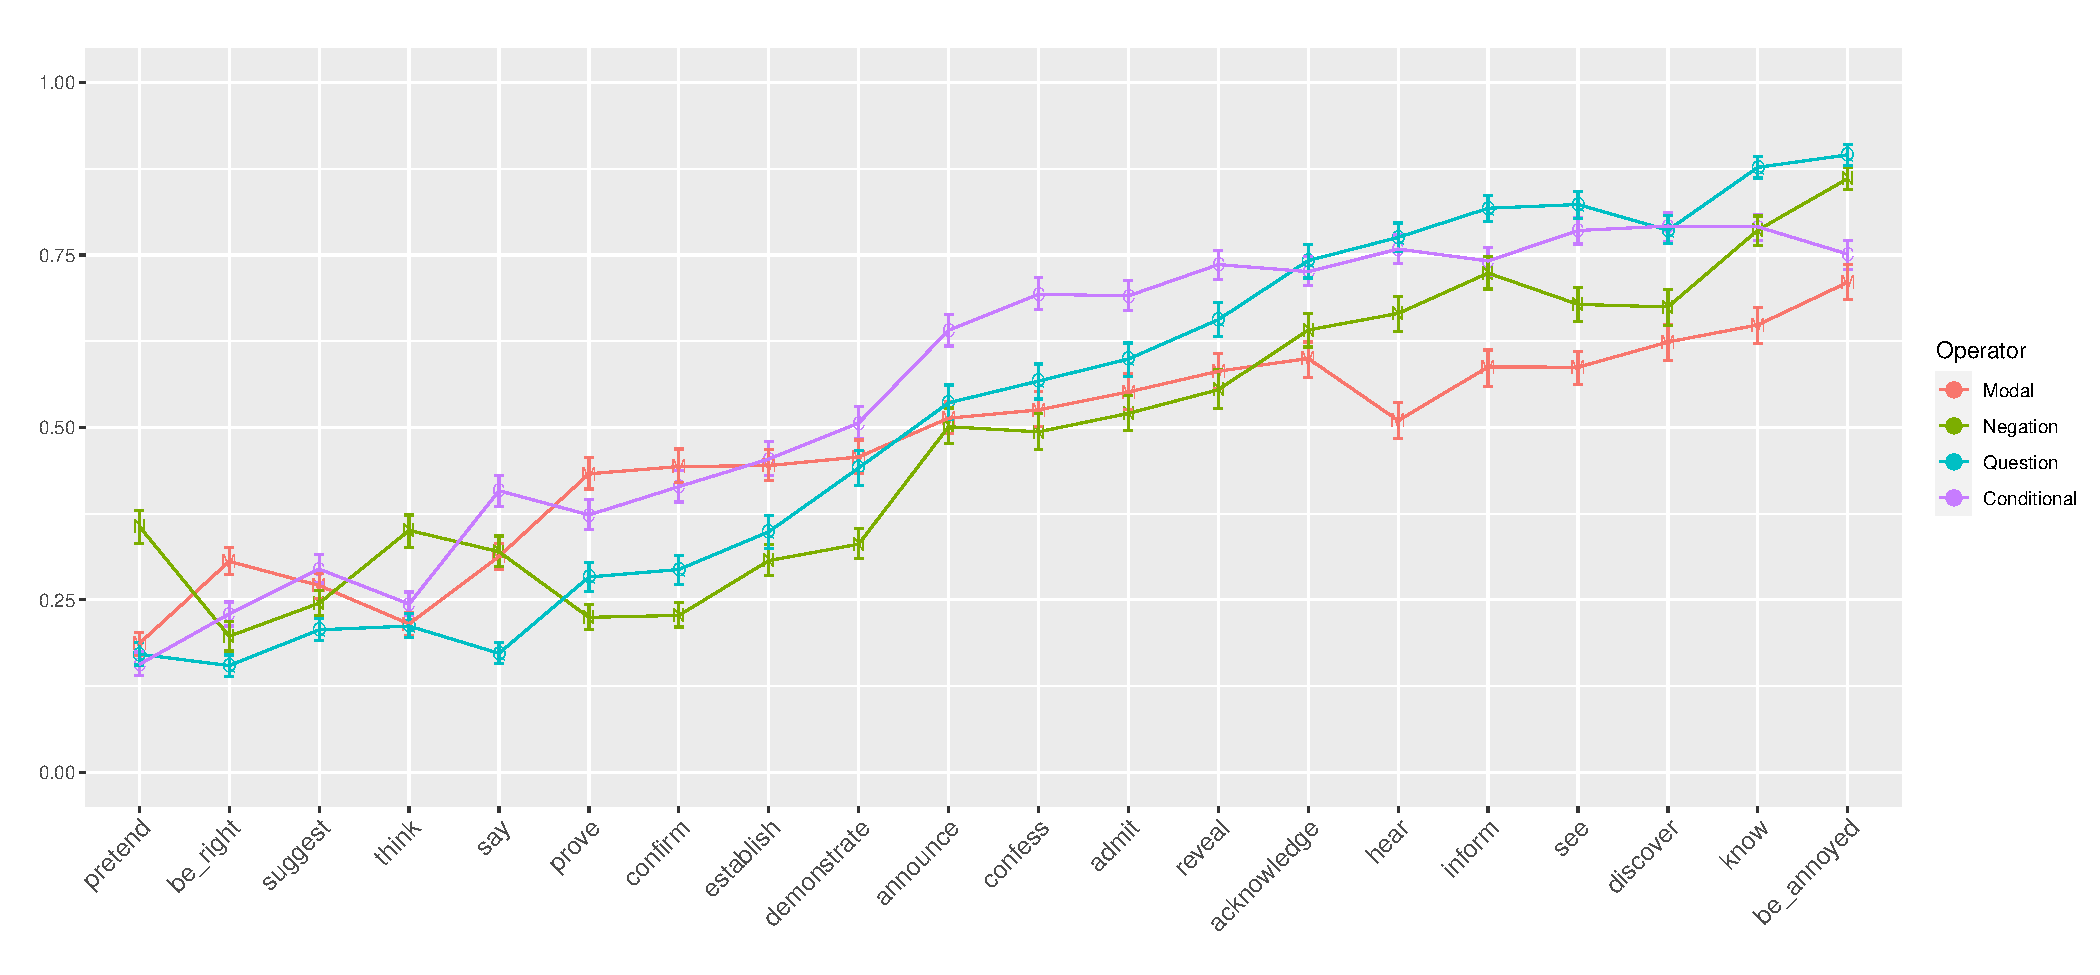
\includegraphics[width=\textwidth]{graphs/proj-by-both.pdf}
		\caption{Mean certainty ratings by operator and predicate}
		\label{fig:figure1}
	\end{figure}

	\begin{itemize}
		\item The embedding operator affects projection (main effect of embedding operator)
		\item This effect differs by verb (interaction effects of operator/verb)
	\end{itemize}
% paragraph method (end)

\paragraph{Discussion and Conclusion.} % (fold)
	\dots
% paragraph method (end)

\pagebreak
\bibliography{projective.bib}

\end{document}